\documentclass[a4paper]{report}
\usepackage{graphicx}

\title{Design of Nqood, a Digital Wallet}
\author{
    Yazeed AlKhalaf \\
    Nawaf Alamer  \\
    Abdullah Meraj \\
    Mohammed Bin Jebreen \\
    Ali Bawazeer \\
    \\
    \textbf{Course:} SWE 300 - Software Processing and Modeling \\
    \textbf{Instructor:} Dr. Ahmed Ghoneim
}
\date{21 Feb, 2024}

\begin{document}

\maketitle

\newpage

\tableofcontents

\chapter*{Abstract}

There are a few applications in the market that allow the user to own both fiat and crypto currencies in one account. Our app aims to fill this gap and offer a great experience to the customers. The revolutionary digital wallet, Nqood, provides all the services for the user through a mobile app, without the need to physical contact. The digital wallet allows users to deposit money in both fiat and crypto currencies seamlessly. The system strikes a balance between great user experience and adhering to the government regulations for protecting user’s data through the usage of NAFATH. The system uses Focal from Mozn which uses AI to provide a highly accurate risk assessment about the individual before onboarding them. It does that while protecting the user’s privacy.

Nqood is a one stop solution to problems faced by people in their everyday life regarding financial transactions. Users can view and pay their bills, traffic violations, SADAD, and government payments, all from one place. They can also automate the payment of those bills. We also provide Apple Pay, madaPay as well as a physical card option. Users can benefit from the 2\% cashback on all their purchases. The spending habits of the user are passed through a GPT model along with their other account data so that the user can ask about and manage his/her account easily using natural language, in any language. The user’s data is protected and never used for training the models.

\chapter{Big Picture}

\begin{figure}[h!]
    \centering
    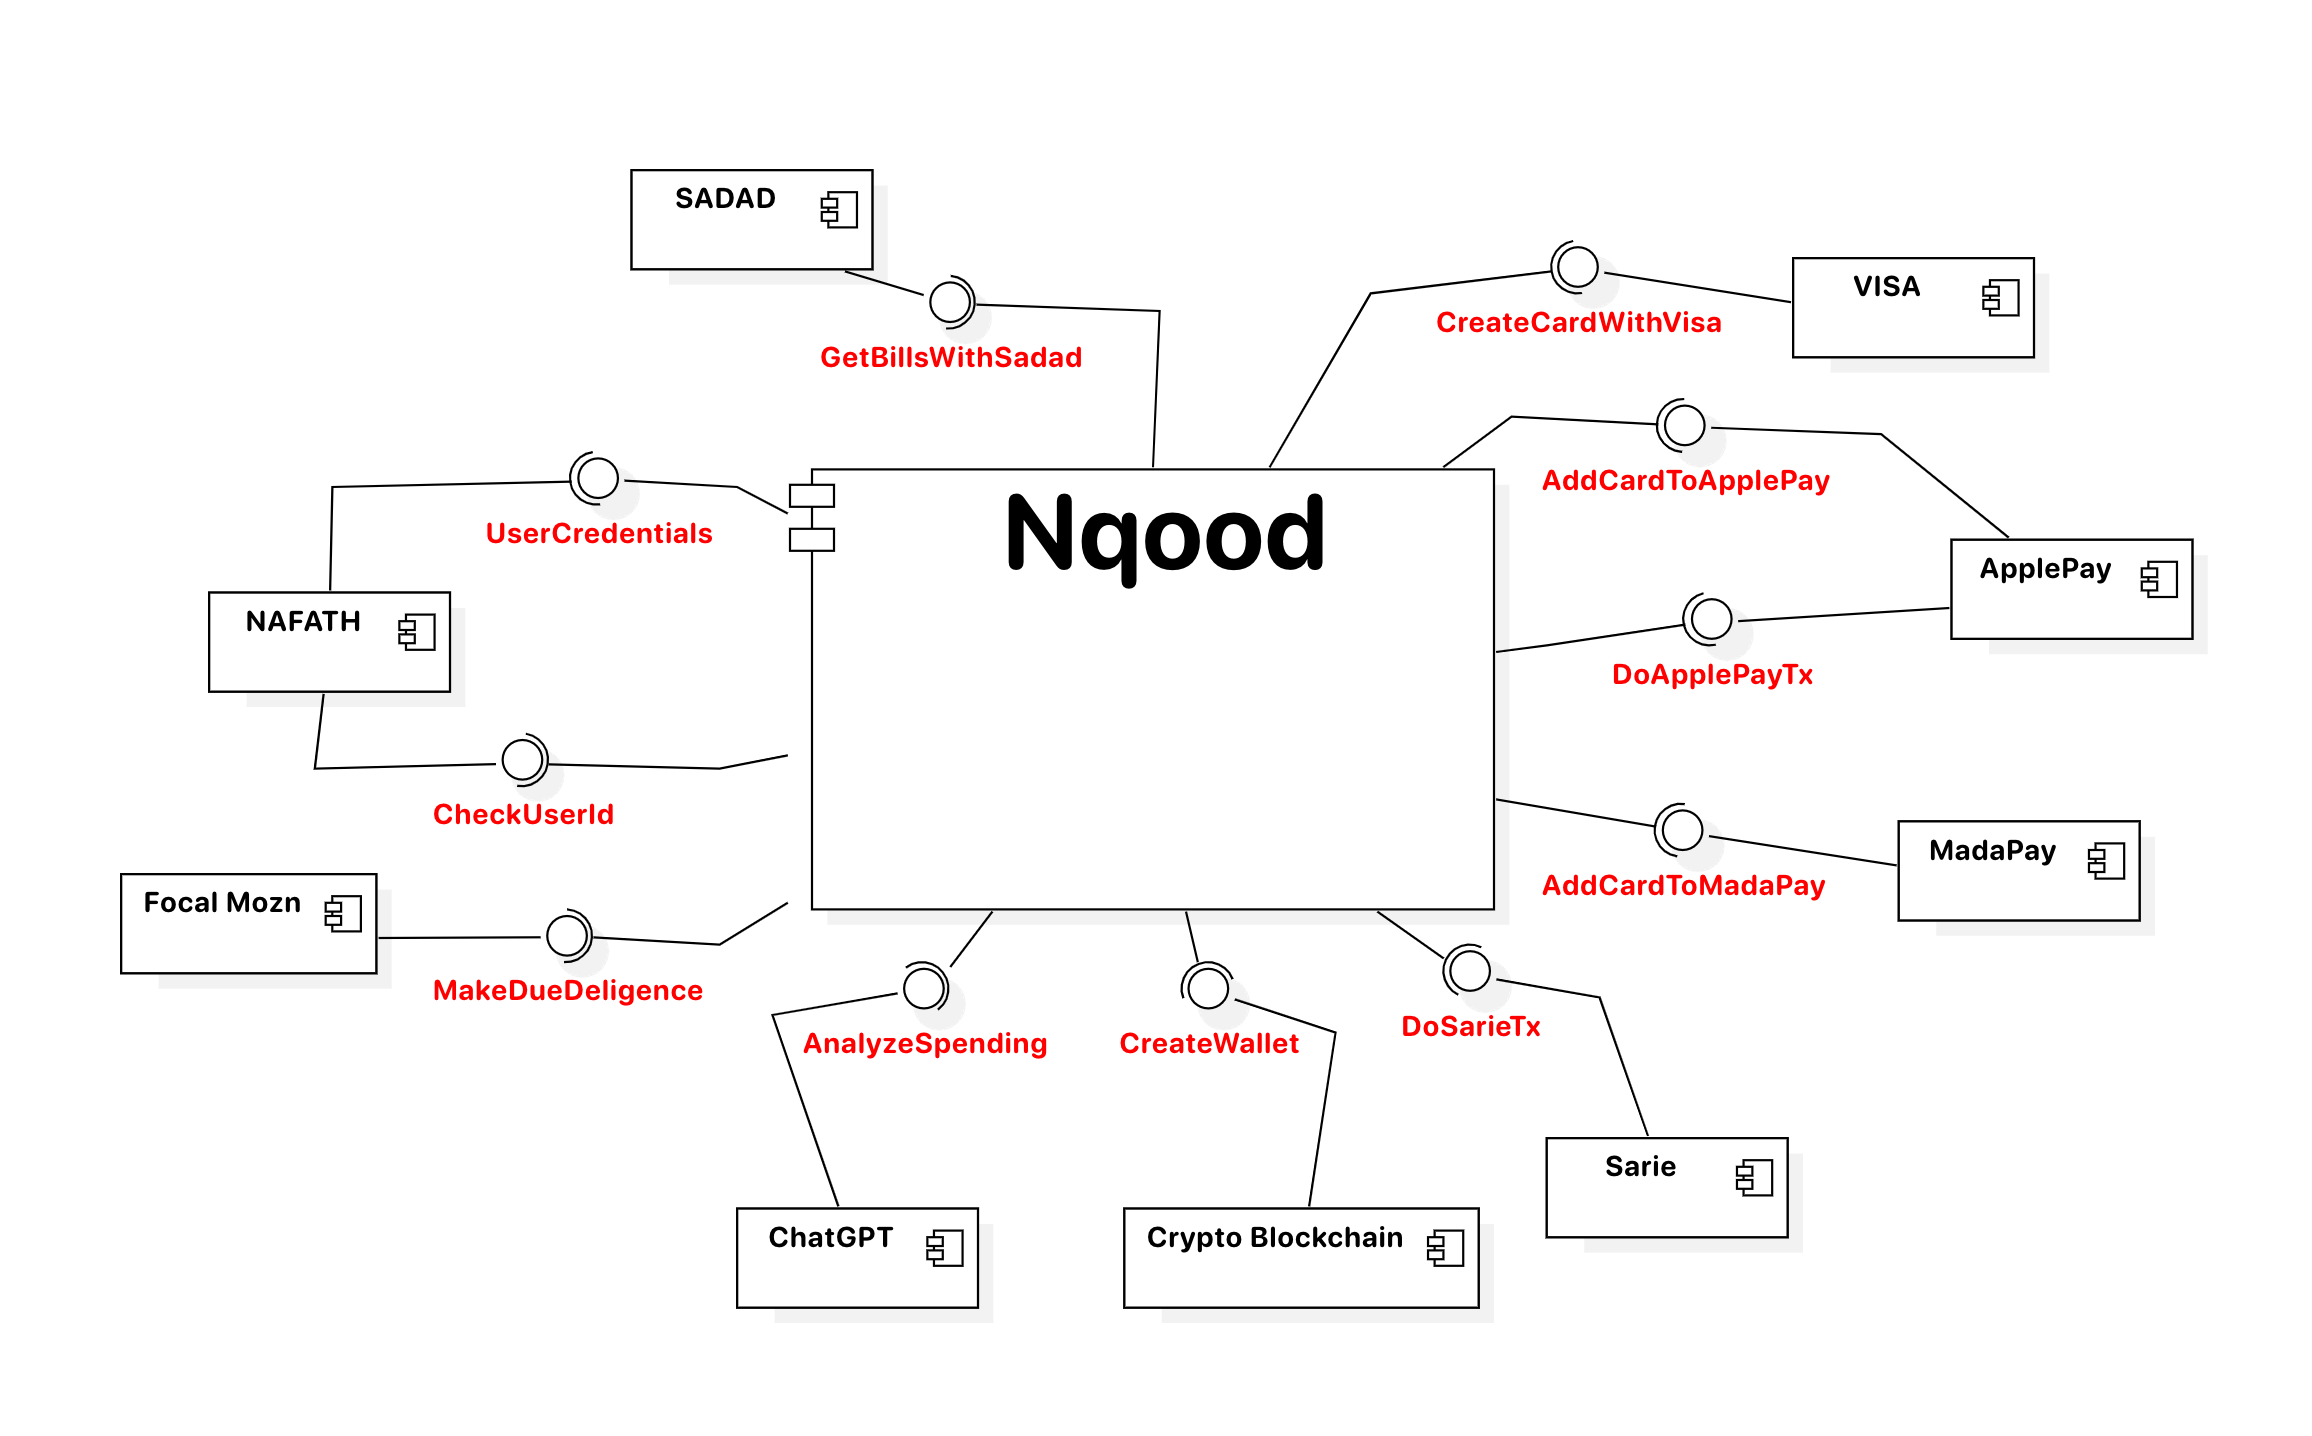
\includegraphics[width=0.8\textwidth]{images/nqood-big-picture.png}
    \caption{Nqood Big Picture}
    \label{fig:big-picture}
\end{figure}

Figure \ref{fig:big-picture} elaborates how the Nqood system communicates with all the external systems. It shows how the frontend receives the information from the backend which collects it from different sources.

\chapter{Black Box}

\begin{figure}[h!]
    \centering
    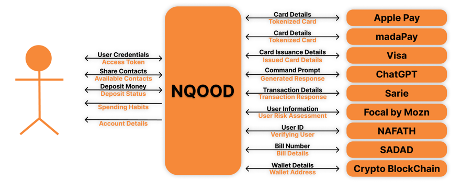
\includegraphics[width=0.8\textwidth]{images/nqood-black-box.png}
    \caption{Nqood Black Box}
    \label{fig:black-box}
\end{figure}

Figure \ref{fig:black-box} demonstrates all the possible inputs and outputs of both a Nqood user and the external systems. Below is a more detailed description of each input/output combination:

\begin{enumerate}
    \item \textbf{Nqood User to Nqood:}
          \begin{enumerate}
              \item The user provides their credentials to Nqood and they get an access token that authenticates and authorizes them.
              \item It gives the option to share the contacts. If the contacts are shared by the user, Nqood will return the available contacts, people who have a Nqood wallet.
              \item Users can get their spending habits after using the wallet for a period.
              \item Users can get their account details, which include account number, balance, and transactions.
              \item Nqood system provides the option for the user to deposit their money through both fiat (Apple Pay, card) and crypto (Bitcoin, Ethereum, etc…) currencies.
          \end{enumerate}
    \item \textbf{Nqood to External Systems:}
          \begin{enumerate}
              \item Nqood tokenizes the card of the user with Apple Pay/madaPay by sending the info to Apple, and then receiving a tokenized card.
              \item Nqood system can talk to Visa to issue a card by providing some Card Issuance Details and receiving an Issued Card Details.
              \item Nqood system can get GPT responses from our fine-tuned GPT by calling the OpenAI API that offers ChatGPT with a “Command Prompt” and receiving a generated response.
              \item Nqood system can transfer money to local banks in Saudi Arabia using Sarie by providing some “Transactoin Details” and receiving a “Transaction Response”. This “Transaction Response” tells whether the transaction was successful or not along with providing some metadata about the transaction.
              \item Nqood system uses the Focal system by Mozn to filter users who are candidates for onboarding. The Focal system uses an advanced AI model to give a risk score along with a full risk assessment that helps compliance in taking the correct action. Nqood sends some user information to Focal which responds with that user’s “Risk Asessment”.
              \item Nqood system uses NAFATH to verify that the user is truly himself trying to open a Nqood wallet. This is a requirement from the regulator SAMA (Saudi Arabian Monetary Authority). Nqood system send the ID of the user and the user must approve this request by taking some action on their personal device that includes biometrics scanning.
              \item Nqood system leverages SADAD services to provide users with bill payment options. Nqood sends the bill number to get the “Bill Details”. The user can take further actions like paying the bill.
              \item Nqood creates a wallet for the user on a crypto blockchain with some “Wallet Details” and saves the address returned by the blockchain and the private key used for the user to manage their newly created wallet.

          \end{enumerate}
\end{enumerate}

\chapter{Design Concrete Component Diagram}

\begin{figure}[h!]
    \centering
    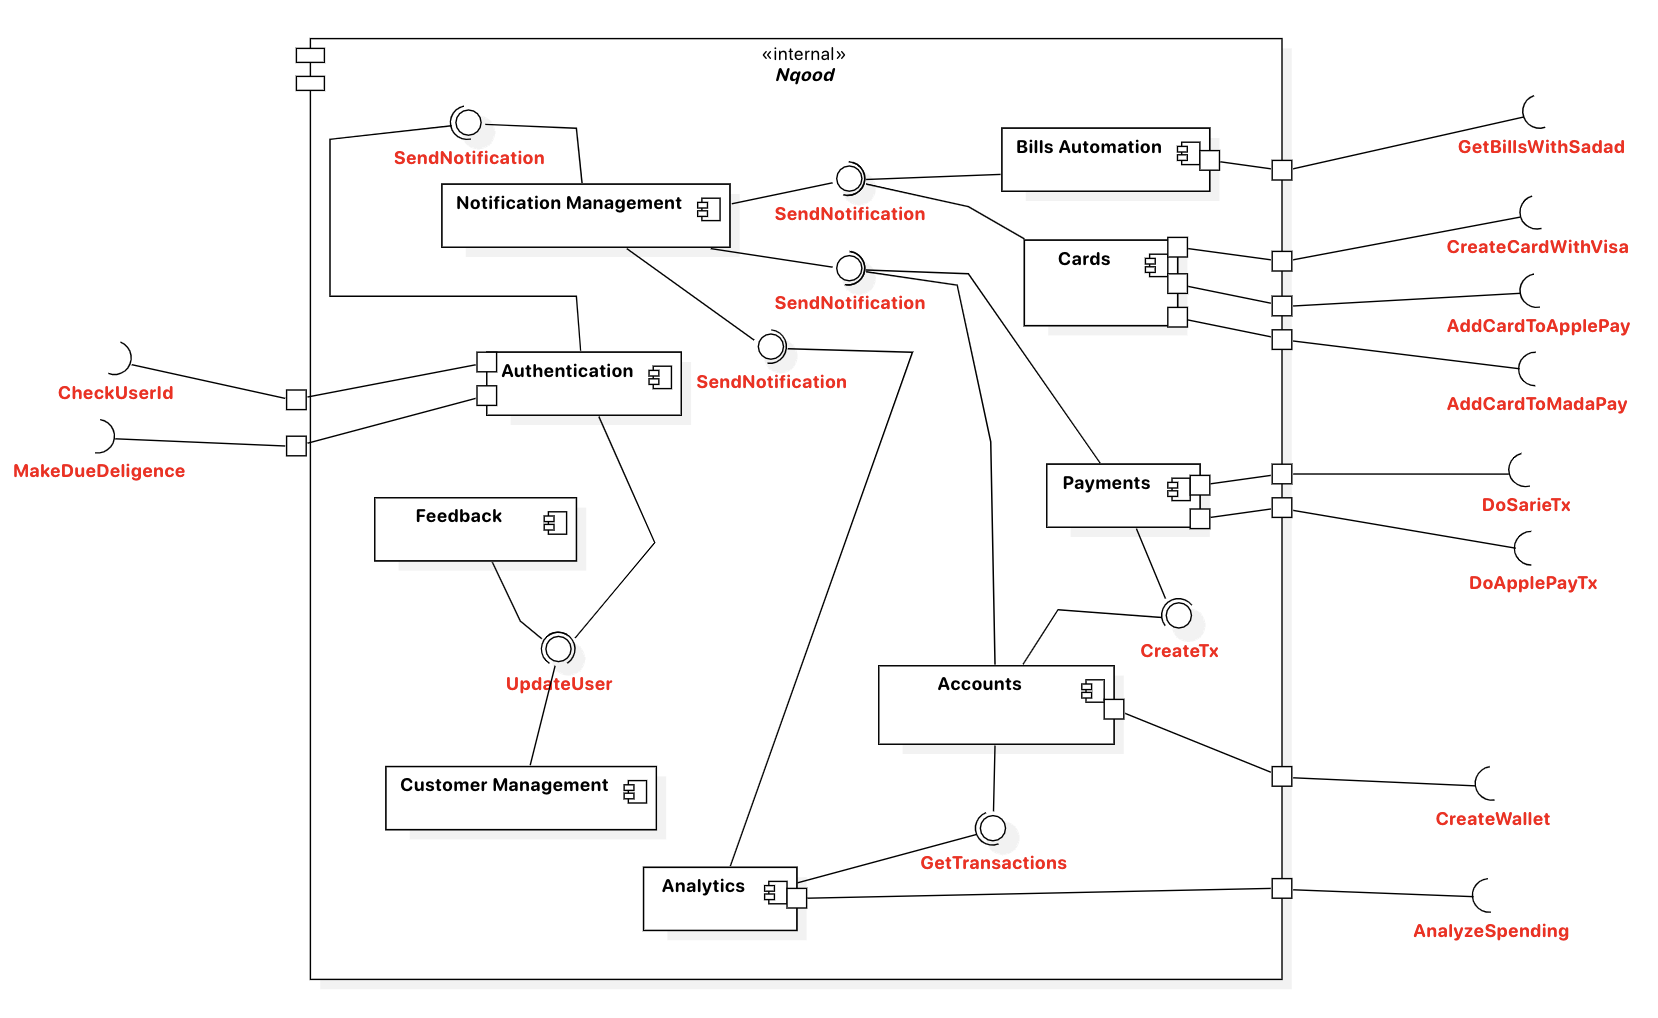
\includegraphics[width=0.8\textwidth]{images/nqood-concrete-component-diagram.png}
    \caption{Nqood Concrete Component Diagram}
    \label{fig:concrete-diagram}
\end{figure}

Figure \ref{fig:concrete-diagram} illustrates how the Nqood system has many external dependencies managed by internal subsystems that make the wallet functionality possible.

Each internal subsystem in the Nqood system has its own database to make each subsystem independent. Below is a description of the 9 internal subsystems:

\begin{enumerate}
    \item \textbf{Accounts:} The accounts subsystem manages the customer accounts user for keeping track of each customer’s money and internal accounts used for keeping a safeguard. It also keeps track of the balances in each account. This system does reconciliation to make sure that the money is not lost.
    \item \textbf{Analytics:} Our analytics internal subsystem provides users with monthly insights into their spending habits, allowing them to track expenses in categories like dining out, transportation, and groceries. It offers appealing data visualization for informed budgeting and lifestyle decisions.
    \item \textbf{Payments:} This subsystem keeps track of all transaction attempts, even if they didn’t succeed. It allows for auditing and preventing fraud by monitoring customers’ behavior. It also serves to make sure reconciliation amounts are correct in the Accounts subsystem.
    \item \textbf{Cards:} The card management system keeps track of the various user cards and sends a notification to the user once the card expires. It also manages the rewards and points of different cards. The subsystem communicates with three external subsystems: VISA, Apple Pay, and madaPay, and to issue cards, and tokenize them respectively.
    \item \textbf{Authentication:} The authentication subsystem handles onboarding and logging in users. It depends on NAFATH and Focal by Mozn to make the onboarding experience safer. The first flow, which is onboarding, creates a customer using the Customer Management subsystem on its success. The second flow allows users to login to their existing accounts by checking with the Customer Management subsystem whether their provided credentials are correct or not.
    \item \textbf{Customer Management:} The customer management system keeps track of the user details and updates them throughout the system as requested by the users.
    \item \textbf{Feedback:} This subsystem allows users to submit feedback about their experience and submit ratings. Then it will be stored in the feedback internal system. This is done to improve the user's experience.
    \item \textbf{Bills Automation:} Bill automation can be activated by the user to pay recurring bills and payments, like utility bills, SADAD bills, traffic violations, and internet/phone bills.
    \item \textbf{Notification Management:} Sends notifications about any changes happening on the account, using SMS, Email, or/and mobile notifications. Users also get notified on transactions, balance changes, card issuance.
\end{enumerate}

\chapter{Nqood Methodology}

\begin{figure}[h!]
    \centering
    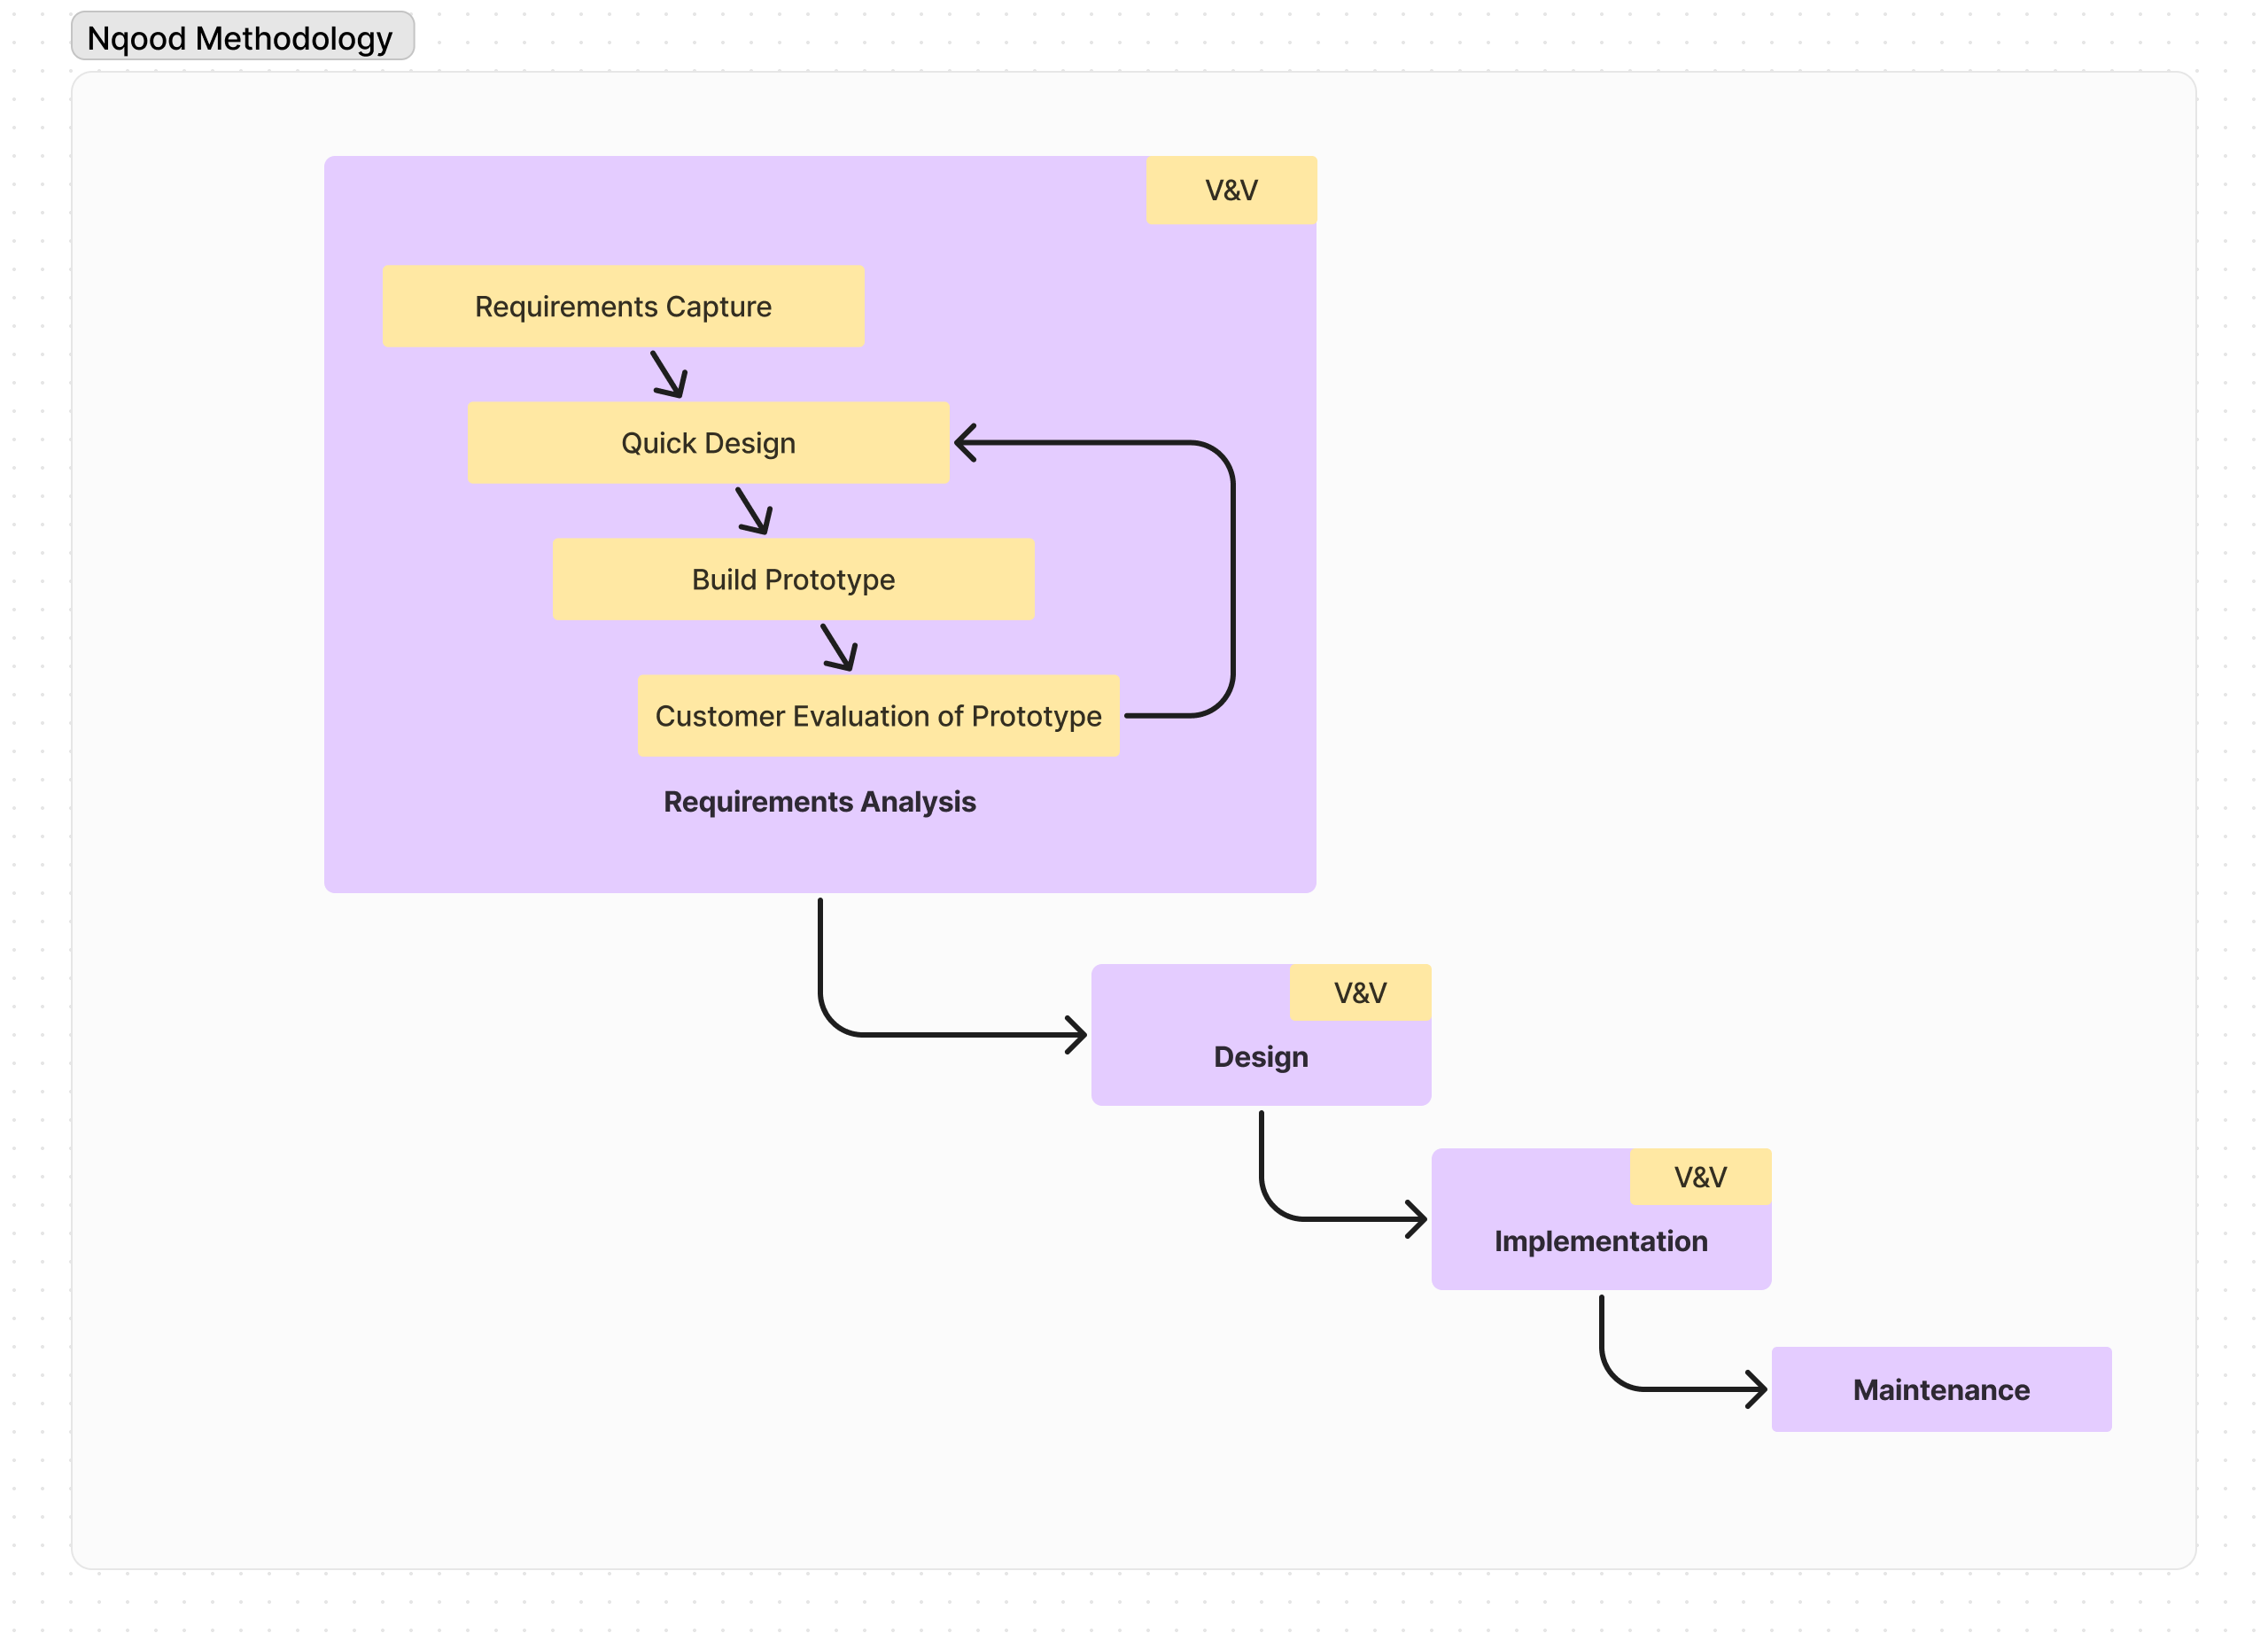
\includegraphics[width=0.8\textwidth]{images/nqood-methodology.png}
    \caption{Nqood Methodology}
    \label{fig:nqood-methodology}
\end{figure}

As seen in Figure \ref{fig:nqood-methodology}, we chose the waterfall model. In industries with strict regularity compliance the waterfall's
document focused approach can be beneficial. It insures that all requirements are documented, implemented and tested
throughly.

We injected prototyping in the requirements phase because we have complex requirements. Waterfall is the best methodology if there are well-defined requirements.

And in every phase we added a V\&V stage. We care a lot about Quality. Quality is important when building a secure and elegant digital wallet. If we don't bake the quality in, we won't have a great product!

\chapter{Iteration 2}

\section{Use Case Diagram for Accounts Subsystem}

\begin{figure}[h!]
    \centering
    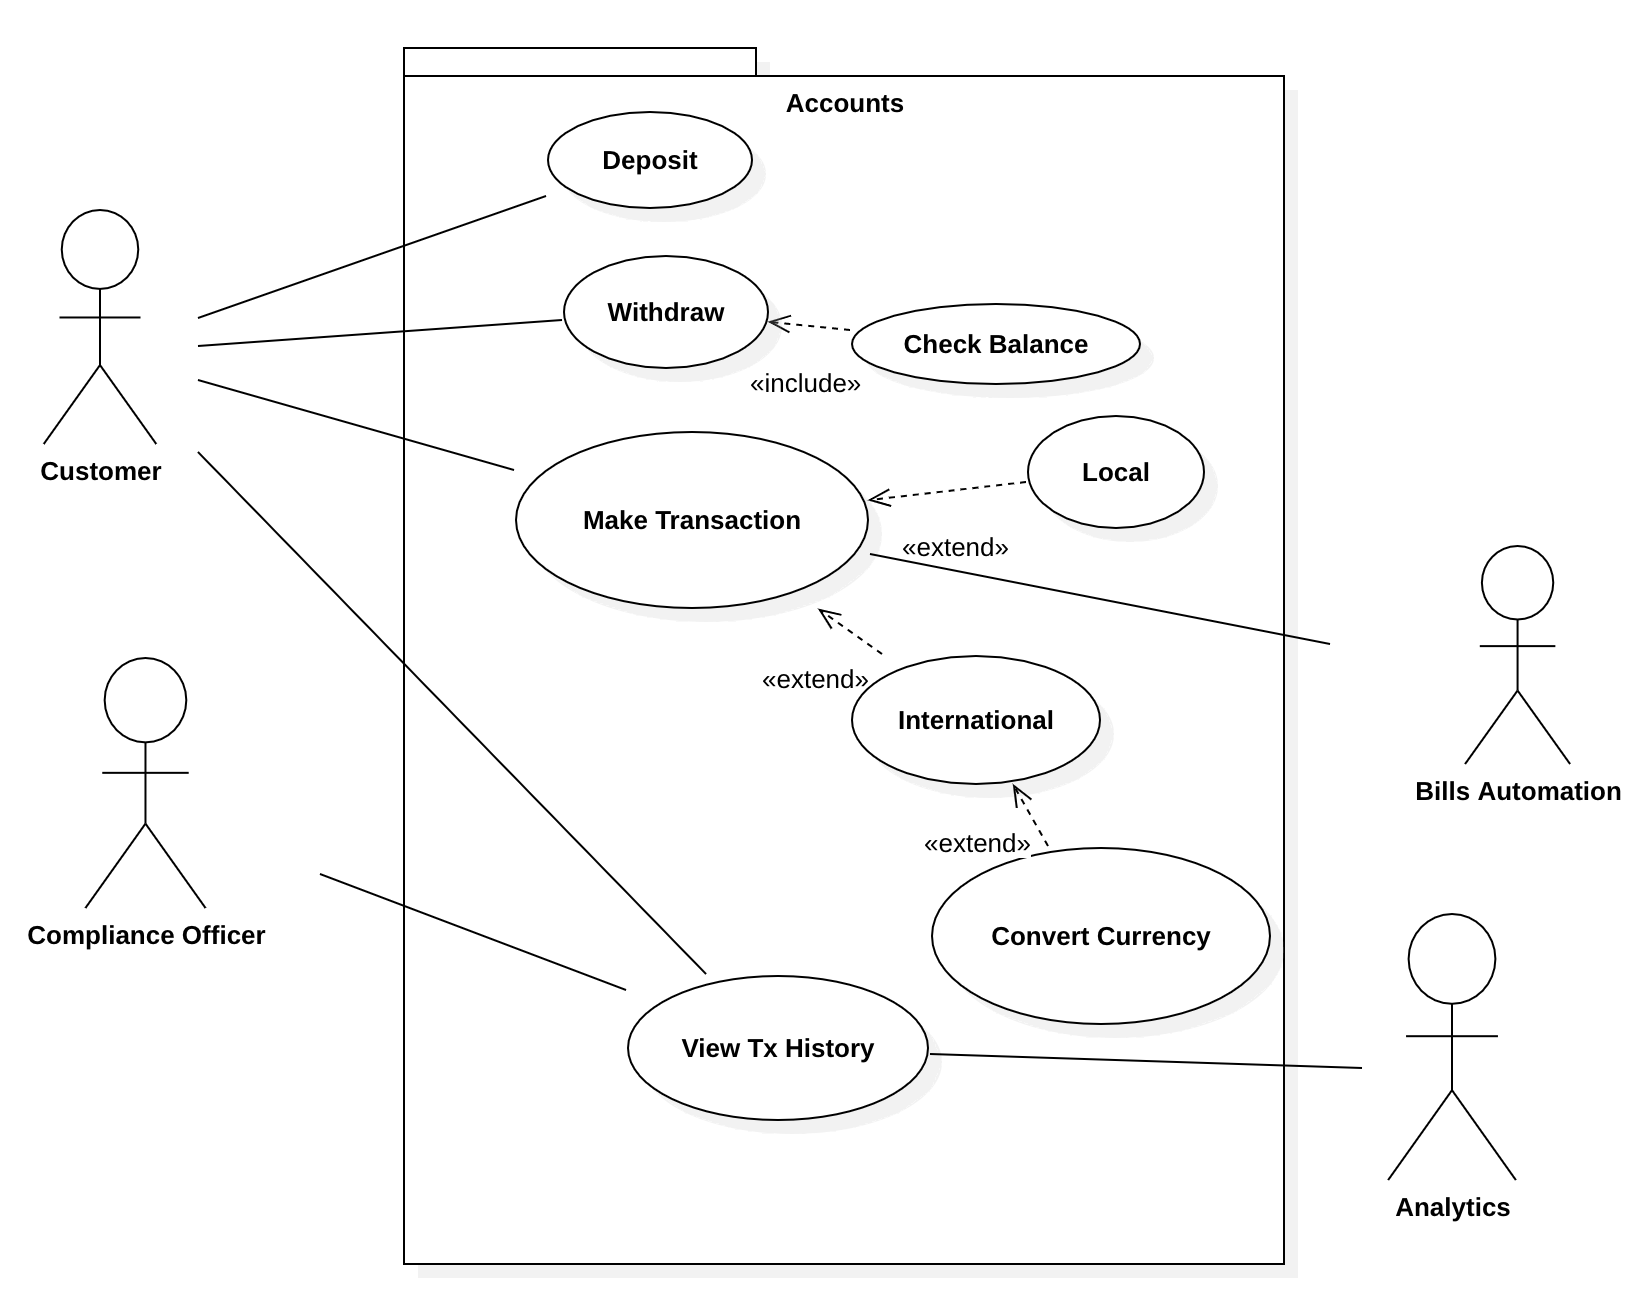
\includegraphics[width=0.8\textwidth]{images/nqood-accounts-use-case-diagram.png}
    \caption{Nqood Accounts Use Case Diagrm}
    \label{fig:nqood-accounts-use-case-diagram}
\end{figure}

\section{Make Transaction Use Case Description}



\section{Make Transaction Use Case Class Diagram}

\begin{figure}[h!]
    \centering
    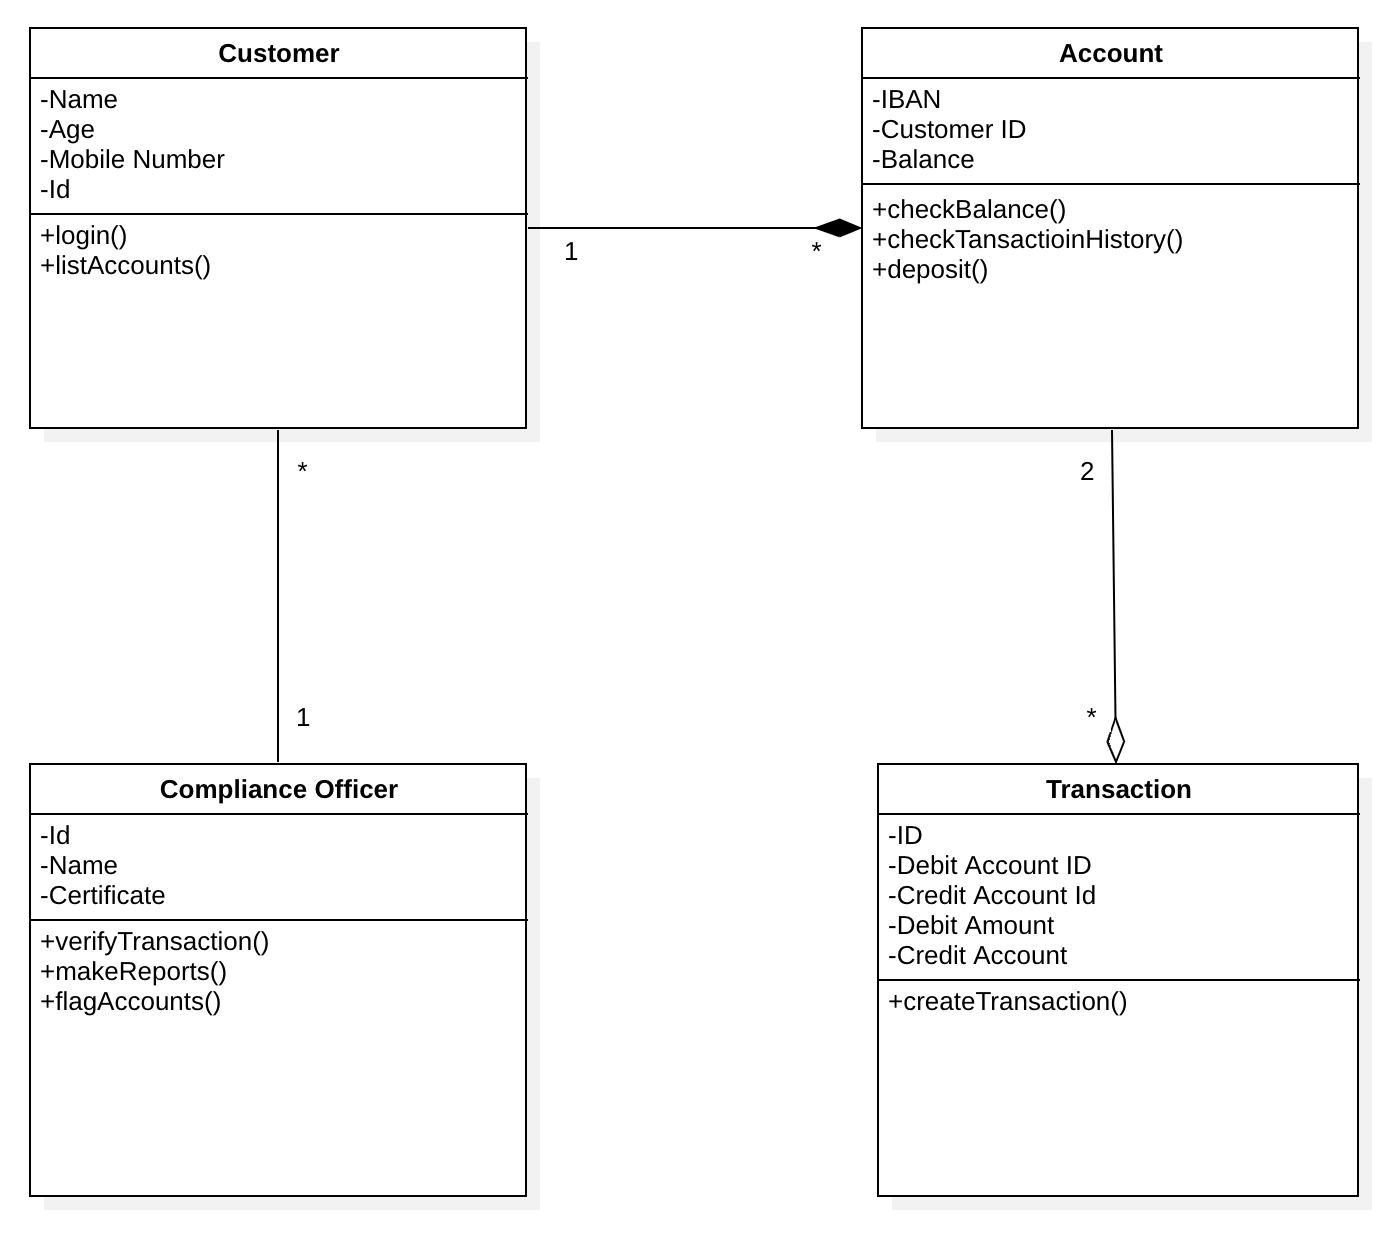
\includegraphics[width=0.8\textwidth]{images/nqood-make-tx-use-case-class-diagram.png}
    \caption{Nqood Make Transaction Use Case Class Diagrm}
    \label{fig:nqood-make-transaction-use-case-class-diagram}
\end{figure}

\end{document}
